\documentclass[11pt]{article}

\usepackage[utf8]{inputenc}
\usepackage[spanish]{babel}
\usepackage[T1]{fontenc}
\usepackage{graphicx}
\usepackage{hyperref}
\usepackage{amsmath}
\usepackage{booktabs}
\usepackage{geometry}
\geometry{margin=2.5cm}

\title{Guía N\textsuperscript{o}2: Paralelismo Local y Procesamiento Distribuido en Data Science}
\author{INFB6074 -- Infraestructura para Ciencia de Datos \\ Universidad Tecnológica Metropolitana (UTEM) \\ Nombre del/los integrante(s): \_\_\_\_\_\_\_\_\_\_\_\_\_\_\_\_\_\_\_\_\_\_}
\date{2026-2}

\begin{document}

\maketitle
\tableofcontents
\newpage

% ---------------------------------------------------------------------------
\section{Portada}

Los datos de portada (integrantes, carrera, fecha de entrega, docente) se
completan en el bloque \texttt{\textbackslash author} y \texttt{\textbackslash date}
anteriores. Ver también el repositorio de entrega para la version en
Markdown de este resumen (\texttt{README.md} en la raíz de \texttt{guia-2/}).

% ---------------------------------------------------------------------------
\section{Resumen ejecutivo}

Este informe documenta cuatro experimentos sobre paralelismo y
procesamiento distribuido aplicados a cargas de trabajo típicas de ciencia
de datos. Los experimentos A, B y C comparan, sobre un único computador,
ejecución secuencial, paralelismo local (hilos, procesos, vectorización
NumPy) y procesamiento distribuido local con Dask. El experimento D
implementa un clúster virtual de tres nodos (Alpine Linux sobre QEMU) con un
modelo coordinador-worker comunicado por sockets TCP y mensajes JSON, para
el cálculo distribuido del conteo de números primos, y compara tres
escenarios: secuencial, un worker remoto y dos workers remotos. En todos los
casos se midió tiempo de ejecución con \texttt{time.perf\_counter()}, se
calculó speedup y eficiencia cuando el número de unidades de paralelismo
(p) fue identificable, y se verificó la equivalencia de resultados entre
métodos. No se dispuso de GPU en el equipo de desarrollo, por lo que la
comparación se centra en vectorización, multiproceso/multihilo local y
distribución local/remota, como permite el enunciado para equipos sin GPU.

% ---------------------------------------------------------------------------
\section{Marco teórico y fuentes}

El desarrollo completo del marco teórico (secuencial/paralelo/distribuido,
arquitectura de clústeres, virtualización con QEMU, redes virtuales y
reenvío de puertos, SSH/SCP, sockets TCP y serialización JSON,
particionamiento estático/dinámico, métricas de speedup/eficiencia/ley de
Amdahl, escalabilidad vertical/horizontal, y disponibilidad/fallas) se
encuentra redactado en \texttt{investigacion/README.md}, con referencias
numeradas consistentes con la lista de referencias bibliográficas (sección
\ref{sec:referencias}). Se resumen aquí solo las definiciones operativas
usadas en el diseño experimental:

\begin{itemize}
  \item \textbf{Secuencial}: una única unidad de ejecución activa.
  \item \textbf{Paralelo de datos}: misma operación sobre particiones distintas de un conjunto de datos (Experimento A).
  \item \textbf{Paralelo de tareas}: tareas independientes, posiblemente distintas entre sí (Experimento B).
  \item \textbf{Distribuido}: nodos/procesos sin memoria compartida, que colaboran mediante paso de mensajes y asumen un costo explícito de comunicación (Experimento D; Dask local en modo \emph{threaded} del Experimento C no cumple esta condición de independencia física, solo la lógica de datos particionados).
  \item \textbf{Speedup y eficiencia}: $S(p) = T_{secuencial}/T_{distribuido}(p)$, $E(p) = S(p)/p$.
  \item \textbf{Ley de Amdahl}: $S(p) \le \dfrac{1}{f + (1-f)/p}$, con $f$ la fracción no paralelizable del trabajo.
\end{itemize}

% ---------------------------------------------------------------------------
\section{Entorno experimental y variables controladas}

\begin{itemize}
  \item \textbf{CPU}: AMD64 (Family 25, Model 33), arquitectura x86-64.
  \item \textbf{Núcleos lógicos}: 16.
  \item \textbf{CPU (modelo)}: AMD Ryzen 7 5700X, 8 núcleos físicos / 16 hilos.
  \item \textbf{RAM}: 16 GB (17.076.400.128 bytes reportados por \texttt{Win32\_ComputerSystem}).
  \item \textbf{Sistema operativo}: Windows 11 (build 10.0.26200).
  \item \textbf{Python}: 3.9.13.
  \item \textbf{Librerías}: NumPy, Pandas, Matplotlib, Dask (\texttt{dask[dataframe]}), psutil.
  \item \textbf{GPU}: no disponible en el equipo de desarrollo; no se incluye comparación con aceleración GPU, conforme a lo permitido por el enunciado cuando no hay GPU, fundamentando la comparación exclusivamente entre vectorización, multiproceso local y distribución local/remota.
\end{itemize}

Variables controladas entre repeticiones: mismos tamaños de entrada, misma
semilla de generación aleatoria (cuando aplica), mismo número de
repeticiones por configuración (3, salvo que se indique otro valor), y
medición exclusiva del tiempo de cómputo (excluyendo en el Experimento D el
tiempo de arranque de las VMs y de los servicios worker, medido por
separado).

% ---------------------------------------------------------------------------
\section{Diseño de los experimentos A, B y C}

\subsection{Experimento A -- Paralelismo de datos y vectorización}

Transformación aplicada a arreglos aleatorios de 5 tamaños (\(10^4\) a
\(2\times10^7\) elementos): normalización respecto del máximo absoluto,
elevación al cuadrado, raíz cuadrada y suma de agregación. Se compararon
tres implementaciones: Python puro (bucle \texttt{for}), NumPy vectorizado,
y \texttt{multiprocessing.Pool} con partición en chunks (2, 4 y 8
procesos). Se verificó equivalencia numérica entre las tres vías con
\texttt{numpy.allclose} antes de registrar cada medición. Python puro se
omitió para los dos tamaños más grandes por tiempo de ejecución
prohibitivo, documentado explícitamente en el código y en el README del
experimento.

\subsection{Experimento B -- Paralelismo a nivel de tareas}

Veinticuatro lotes independientes de feature engineering (escalado,
encoding one-hot manual, variables derivadas) sobre un DataFrame sintético
de ventas, en 3 tamaños de lote (200, 1000 y 5000 filas) y 2 tipos de carga:
CPU-bound (solo cómputo) e I/O-bound simulada (cómputo más una espera corta
por lote). Se compararon ejecución secuencial, \texttt{ThreadPoolExecutor} y
\texttt{ProcessPoolExecutor}, cada uno con 2, 4 y 8 workers.

\subsection{Experimento C -- Procesamiento distribuido sobre datos particionados}

Dieciséis archivos CSV sintéticos de ventas, particionados por fecha
(\textasciitilde60.000 filas cada uno), leídos con \texttt{dask.dataframe}
bajo 3 configuraciones de particionamiento (4, 8 y 16 particiones lógicas),
con una transformación (monto por unidad) y una agregación
\texttt{groupby(fecha, tienda)}, comparados en tiempo y resultado contra el
equivalente en Pandas puro sobre los mismos datos concatenados en memoria.

% ---------------------------------------------------------------------------
\section{Diseño de la infraestructura virtual del experimento D}

Tres máquinas virtuales Alpine Linux 3.24 (kernel 6.18.62-0-virt, Python
3.14.10) sobre QEMU 11.1.0, con el acelerador \texttt{whpx} del hipervisor de
Windows: nodo0 (coordinador), nodo1 y nodo2 (workers), cada una con 1 vCPU y
512 MB de RAM. Las tres se instalaron de forma desatendida, con el
\emph{answer file} de \texttt{setup-alpine -f} escrito por la consola serial de
QEMU (el procedimiento está en \texttt{experimento-d/scripts/instalar\_nodo.md}).
Red en modo \texttt{user} (NAT) de QEMU, con reenvío de puertos
(\texttt{hostfwd}) para SSH (2220/2221/2222 hacia el puerto 22 de cada VM) y
para el servicio TCP de cálculo (9001/9002 hacia el puerto 9000 interno de
nodo1 y nodo2 respectivamente). El coordinador, corriendo en nodo0, alcanza
a los workers a través del anfitrión, en \texttt{10.0.2.2:9001} y
\texttt{10.0.2.2:9002}.

% ---------------------------------------------------------------------------
\section{Implementación del modelo coordinador-worker y protocolo}

El worker (\texttt{experimento-d/src/worker.py}) escucha en
\texttt{0.0.0.0:9000} (todas las interfaces de la VM) usando
\texttt{socketserver.ThreadingTCPServer}, cuenta números primos en el
intervalo recibido mediante una criba de Eratóstenes, y mide su propio
tiempo de procesamiento con \texttt{time.perf\_counter()}. El protocolo usa
una conexión TCP por solicitud, con mensajes JSON UTF-8 delimitados por
salto de línea:

\begin{verbatim}
Solicitud:  {"start": <int>, "end": <int>}
Respuesta:  {"worker": "<id>", "result": <int>, "processing_seconds": <float>}
\end{verbatim}

El coordinador (\texttt{experimento-d/src/coordinator.py}) lee hasta el
delimitador sin asumir que una sola lectura trae el mensaje completo, limita
el tamaño máximo de mensaje aceptado, y aplica timeout a toda la operación.
Valida tipos, rangos y correspondencia del campo \texttt{worker}; ante
cualquier falla (timeout, conexión rechazada, respuesta malformada), marca
el escenario como incompleto explícitamente, sin bloquear la ejecución ni
presentar un resultado parcial como si fuera el total. El particionamiento
estático entre $N$ workers se calcula con una función genérica que garantiza
cobertura completa del intervalo sin huecos ni solapamientos.

Esta implementación fue verificada de extremo a extremo en modo
\emph{simulación local} (dos procesos \texttt{worker.py} en \texttt{localhost},
lanzados y detenidos automáticamente por
\texttt{coordinator.py simulacion}), confirmando el correcto funcionamiento
del protocolo antes de ejecutarlo contra las VMs reales.

% ---------------------------------------------------------------------------
\section{Resultados experimentales y verificación de correctitud}

\subsection{Experimentos A, B y C}

Los resultados completos están en
\texttt{experimento-a/evidencias/resultados\_a.csv},
\texttt{experimento-b/evidencias/resultados\_b.csv} y
\texttt{experimento-c/evidencias/resultados\_c.csv}. En los tres casos se
verificó programáticamente la equivalencia de resultados entre métodos antes
de registrar las mediciones (\texttt{assert} en el código de cada
experimento), por lo que ninguna fila de estos CSV corresponde a una
ejecución con resultado numérico divergente entre métodos.

\textbf{Experimento A.} NumPy vectorizado gana en los cinco tamaños, sin
excepción: 33~$\mu$s para $10^4$ elementos y 0,165~s para $2\times10^7$,
creciendo de forma aproximadamente lineal con el tamaño. Python puro
(disponible hasta $10^6$, omitido después por tiempo prohibitivo) va de
1,17~ms a 0,117~s, es decir unas 15 veces más lento que NumPy en $10^6$.
\texttt{multiprocessing} no gana en ningún tamaño probado: su tiempo arranca en
0,53~s para $10^4$ y llega a 0,78~s para $2\times10^7$, porque está dominado
por un costo fijo de arranque de procesos de medio segundo (en Windows, cada
proceso se crea por \emph{spawn}, reimportando el intérprete). El speedup
respecto de NumPy sube de 0,0001 a 0,21 al crecer el problema --la tendencia es
la correcta-- pero nunca cruza el 1, y \emph{empeora} al agregar procesos:
0,21 con 2 procesos, 0,208 con 4 y 0,177 con 8 para el tamaño mayor. Más
procesos significan más overhead de creación sin más trabajo útil que repartir.

\textbf{Experimento B.} El resultado depende por completo del tipo de carga.
Con trabajo CPU-bound, la ejecución secuencial (0,046--0,065~s según el tamaño
de lote) es la mejor opción: los hilos empatan (0,044--0,080~s, sin ganancia
real, como corresponde a un intérprete con GIL donde el cómputo no lo libera) y
los procesos son entre 15 y 20 veces peores (0,98--1,39~s), otra vez por el
costo de crearlos. Con trabajo I/O-bound la figura se invierte: sobre una
referencia secuencial de 0,73--0,75~s, los hilos escalan casi linealmente hasta
8 workers --0,374~s con 2 ($1,96\times$), 0,193--0,204~s con 4
($\approx3,7\times$) y 0,114--0,139~s con 8 ($5,4\times$ a $6,4\times$)--,
mientras que los procesos siguen siendo peores que no paralelizar
(1,23--1,47~s). El GIL se libera durante la espera de I/O, y ahí los hilos
sirven; en cómputo puro, no.

\textbf{Experimento C.} Dask supera a Pandas puro en las tres configuraciones,
con un óptimo intermedio: 0,569~s en Pandas contra 0,273~s con 4 particiones
($2,09\times$), 0,268~s con 8 ($2,13\times$) y 0,364~s con 16 ($1,56\times$).
Pasar de 8 a 16 particiones \emph{empeora} el tiempo: el costo de planificar y
coordinar más tareas supera lo que se gana dividiendo más. Las cuatro
configuraciones devuelven las mismas 64 filas de la agregación, que es la
comprobación de que la partición no alteró el resultado.

\subsection{Experimento D}

La batería se ejecutó \textbf{en nodo0}, el coordinador, contra los workers de
nodo1 y nodo2: cinco tamaños de intervalo, tres escenarios y tres repeticiones
cada combinación, 45 mediciones en total
(\texttt{experimento-d/evidencias/resultados\_d.csv}).

\textbf{Correctitud.} La prueba previa (contar primos en $[2,10]$, esperado 4)
dio 4 en los tres escenarios: local sin red, un worker remoto y dos workers
remotos. Para cada uno de los cinco tamaños, los tres escenarios completos
coincidieron en el resultado: 1.229, 9.592, 41.538, 148.933 y 664.579 primos
para $10^4$, $10^5$, $5\times10^5$, $2\times10^6$ y $10^7$ respectivamente
--$\pi(10^7)=664.579$ es el valor conocido de la función contadora de primos,
lo que confirma que la partición y la agregación no perdieron ni duplicaron
nada--. La verificación de que las particiones cubren el intervalo sin huecos
ni solapamientos está en \texttt{evidencias/04\_particion\_y\_parciales.txt}:
para $[2, 500.000]$, nodo1 recibe $[2, 250.001]$ y nodo2 $[250.002, 500.000]$,
250.000 + 249.999 = 499.999 números, exactamente el intervalo.

\begin{table}[h]
\centering
\small
\begin{tabular}{lrrrrr}
\toprule
Escenario & $10^4$ & $10^5$ & $5\times10^5$ & $2\times10^6$ & $10^7$ \\
\midrule
A secuencial (s)   & 0,000082 & 0,000554 & 0,003637 & 0,015178 & 0,083291 \\
B un worker (s)    & 0,002225 & 0,003412 & 0,006998 & 0,024130 & 0,079851 \\
C dos workers (s)  & 0,004273 & 0,003633 & 0,007992 & 0,018112 & 0,074629 \\
\midrule
Speedup B          & 0,048 & 0,189 & 0,563 & 0,649 & \textbf{1,079} \\
Speedup C          & 0,021 & 0,156 & 0,469 & 0,859 & \textbf{1,197} \\
Eficiencia C       & 0,010 & 0,078 & 0,234 & 0,430 & 0,598 \\
\bottomrule
\end{tabular}
\caption{Experimento D: tiempo total medio de las tres repeticiones, y speedup
y eficiencia respecto del escenario secuencial. En negrita, los dos únicos
casos en que distribuir resultó más rápido que no distribuir.}
\end{table}

El hallazgo central es \textbf{dónde está el cruce}. En los tres tamaños
menores, distribuir es peor que no distribuir, y con dos workers es peor que
con uno: para $10^4$, el escenario secuencial tarda 82~$\mu$s y el de dos
workers 4,3~ms, 52 veces más. El cálculo es sencillamente demasiado barato --la
criba de Eratóstenes sobre \texttt{bytearray} usa asignación por rebanadas, que
corre a velocidad de C-- frente al costo de hablar por red. Recién en $10^7$ el
cómputo pesa lo suficiente: un worker da speedup 1,08 y dos workers 1,20, y por
primera vez agregar el segundo worker mejora en vez de empeorar. La eficiencia,
en cambio, nunca se acerca a 1 (0,598 en el mejor caso con dos workers): la
mitad del paralelismo se va en coordinación.

% ---------------------------------------------------------------------------
\section{Comparación de rendimiento y visualizaciones}

Gráficos generados por los experimentos A, B y C:
\texttt{experimento-a/evidencias/tiempo\_vs\_tamano.png},
\texttt{experimento-a/evidencias/speedup\_vs\_p.png},
\texttt{experimento-b/evidencias/comparacion\_b.png},
\texttt{experimento-c/evidencias/comparacion\_c.png}.

\begin{figure}[h]
\centering
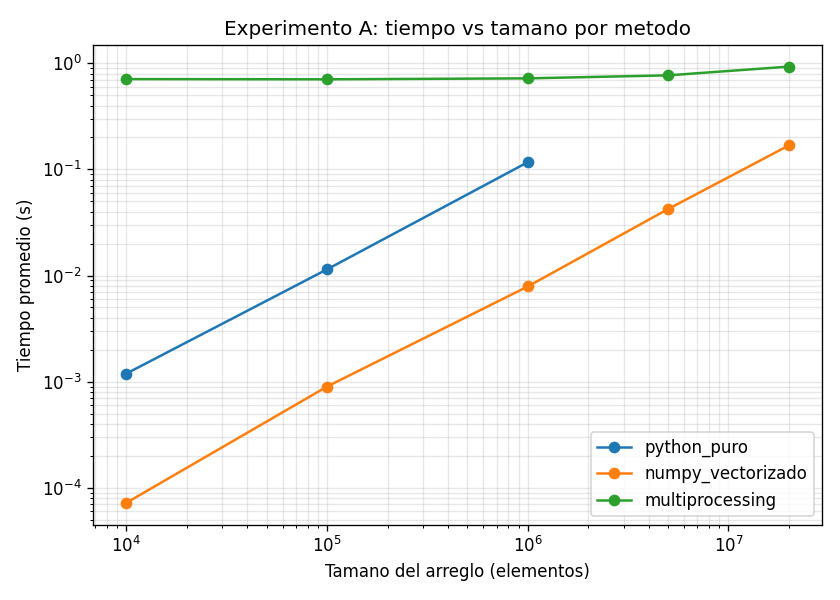
\includegraphics[width=0.49\textwidth]{experimento-a/evidencias/tiempo_vs_tamano.png}
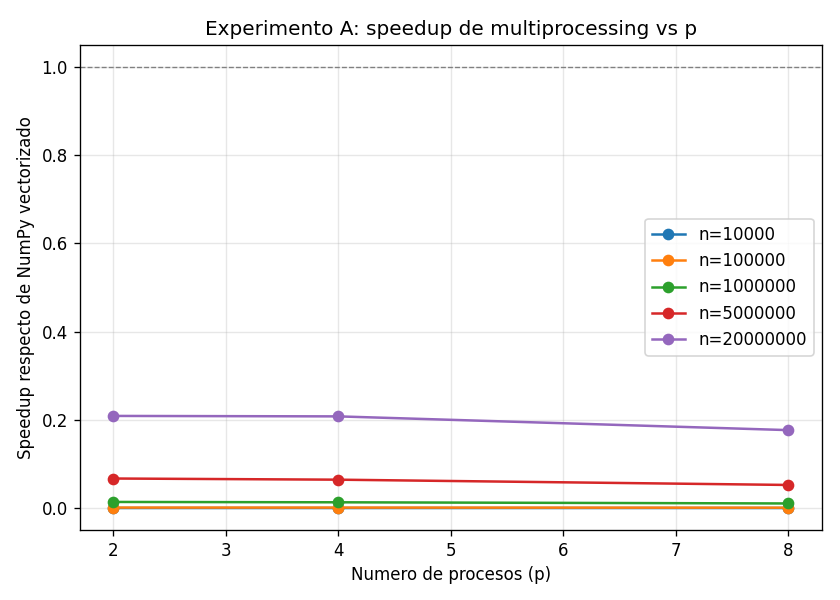
\includegraphics[width=0.49\textwidth]{experimento-a/evidencias/speedup_vs_p.png}
\caption{Experimento A. Izquierda: tiempo contra tamaño de entrada por método.
NumPy queda por debajo de las otras dos curvas en todo el rango y nunca es
alcanzado. Derecha: speedup contra número de procesos; la curva baja en vez de
subir, porque cada proceso adicional agrega costo de creación sin agregar
trabajo útil.}
\end{figure}

\begin{figure}[h]
\centering
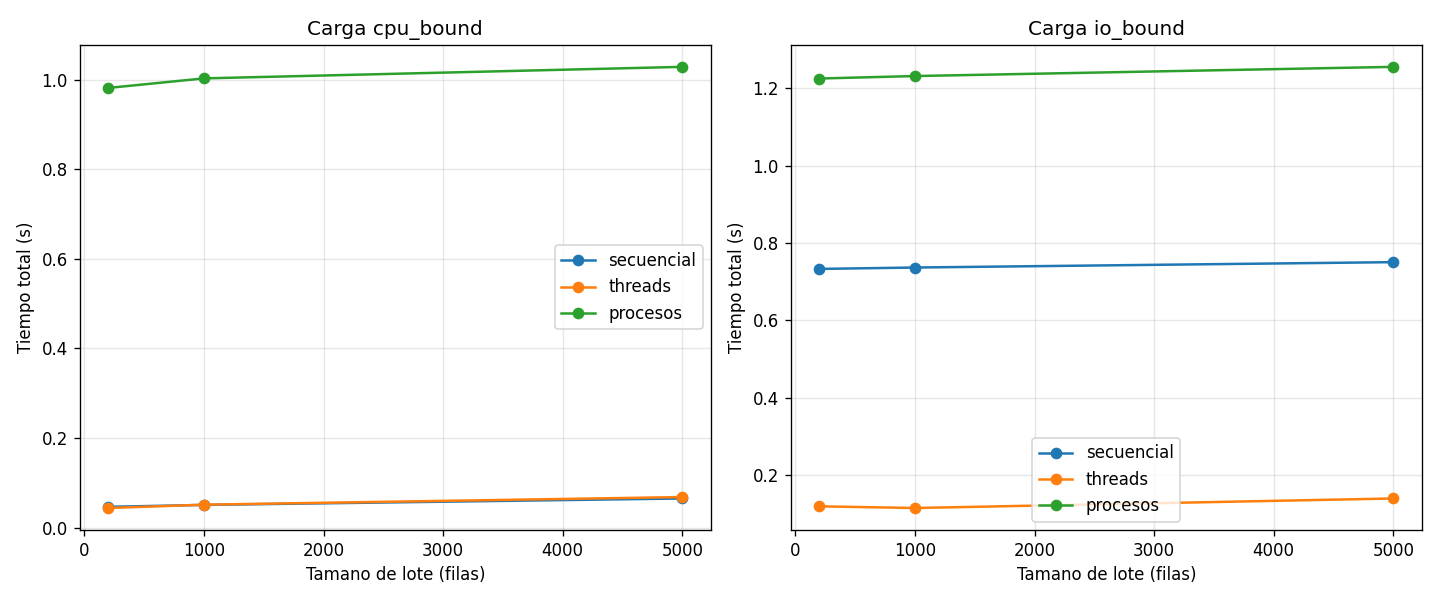
\includegraphics[width=0.49\textwidth]{experimento-b/evidencias/comparacion_b.png}
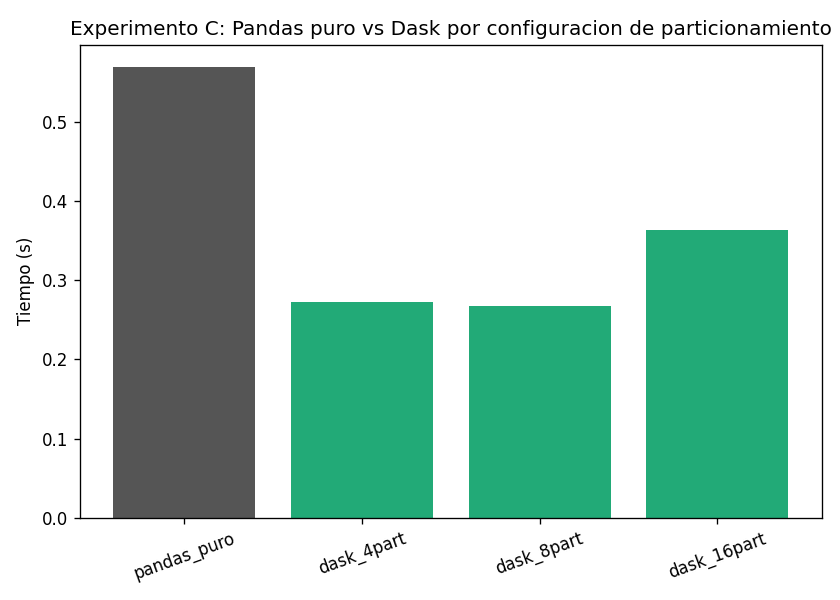
\includegraphics[width=0.49\textwidth]{experimento-c/evidencias/comparacion_c.png}
\caption{Izquierda, Experimento B: hilos y secuencial empatan en CPU-bound (el
GIL no se libera durante el cómputo) mientras que en I/O-bound los hilos
escalan hasta $6\times$; los procesos pierden en ambos casos por el costo de
\emph{spawn}. Derecha, Experimento C: Dask mejora a Pandas puro, con el óptimo
en 8 particiones y una pérdida visible al pasar a 16.}
\end{figure}

\begin{figure}[h]
\centering
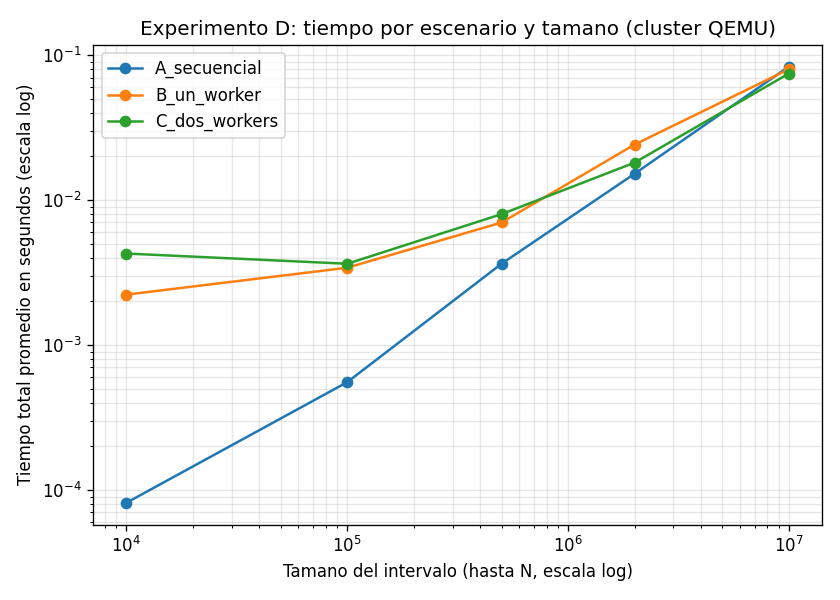
\includegraphics[width=0.72\textwidth]{experimento-d/evidencias/comparacion_d.png}
\caption{Experimento D, sobre el clúster QEMU real. Ejes logarítmicos: en
escala lineal los tres tamaños menores se apilarían sobre el cero, que es justo
el tramo donde el overhead manda. Las curvas de los escenarios distribuidos
tienen un piso plano de 2 a 4~ms --el costo fijo de coordinación, que no
desaparece por más pequeño que sea el problema-- mientras que la secuencial
baja sin límite. Las curvas se cruzan cerca de $10^7$: ahí el cómputo por fin
pesa más que la comunicación.}
\end{figure}

% ---------------------------------------------------------------------------
\section{Análisis de overhead y escalabilidad}

En el Experimento D, el overhead/residual se aproxima como:
\[
  \text{residual} = T_{total,\,distribuido} - \max_i\left(T_{procesamiento,\,worker_i}\right)
\]
magnitud que agrupa preparación, planificación, transferencia y agregación,
sin aislar exclusivamente la latencia de red.

Medido sobre el clúster real, el residual \textbf{no crece con el tamaño del
problema}. Con un worker va de 2,1~ms ($10^4$) a 5,1~ms ($10^7$), y con dos
workers de 4,2~ms a 4,2~ms, pasando por 5,3~ms en $5\times10^5$: la variación
es ruido, no tendencia. Eso es exactamente lo que se espera de un costo fijo
--abrir la conexión TCP, serializar una solicitud de dos enteros, esperar,
deserializar una respuesta corta, sumar-- cuyo tamaño de mensaje es el mismo
tanto si el intervalo tiene diez mil números como diez millones.

La consecuencia práctica es que el residual se vuelve despreciable por división,
no por reducción: en $10^4$ representa el 98\% del tiempo total del escenario
con dos workers, y en $10^7$ apenas el 5,6\%. No se arregla optimizando la red;
se arregla dándole al worker trabajo suficiente como para que valga la pena
haberlo llamado.

Pasar de uno a dos workers aumenta el residual, pero menos que al doble (por
ejemplo, 3,9~ms contra 5,0~ms en $2\times10^6$), porque las dos solicitudes
salen en paralelo desde un \texttt{ThreadPoolExecutor} y el costo que se suma es
el de la segunda conexión, no el de una segunda espera completa.

Sobre la escalabilidad horizontal hay que ser honesto con lo que este montaje
puede y no puede demostrar: las tres VMs comparten el mismo CPU físico y la
misma RAM del anfitrión. Agregar un worker no agrega capacidad de cómputo al
sistema; reparte la que ya hay. El speedup de 1,20 observado en $10^7$ es real
--está medido-- pero proviene de usar dos núcleos físicos del mismo procesador
que de todos modos estaban disponibles, no de haber sumado una máquina. En un
clúster físico, el mismo código tendría el mismo costo de coordinación (o
mayor, con red real) pero cada nodo sí aportaría cómputo propio.

% ---------------------------------------------------------------------------
\section{Análisis de disponibilidad y fallas}

Se diseñó y verificó (en simulación local) que, al detener un worker, el
coordinador detecta la falla por timeout o conexión rechazada, sin bloquearse
indefinidamente, y marca el escenario afectado como incompleto.

La prueba se repitió sobre el clúster real
(\texttt{evidencias/07\_falla\_de\_un\_worker.txt}). Con los dos workers
corriendo, la prueba de correctitud pasó en los tres escenarios. Se detuvo
entonces el servicio en nodo2 (\texttt{pkill -f worker.py}, confirmado con
\texttt{ps}) y se repitió la batería para $5\times10^5$ y $10^7$. El resultado:

\begin{itemize}
  \item El coordinador \textbf{no se bloqueó}: la corrida completa tardó
  0,46~s, muy por debajo del \texttt{TIMEOUT\_SEGUNDOS} de 15~s.
  \item Los escenarios A (secuencial) y B (un worker, el de nodo1) siguieron
  completos y con el resultado correcto: 41.538 y 664.579 primos.
  \item El escenario C quedó marcado \texttt{completo=False}, con el motivo
  registrado en el CSV y el worker identificado:
  \texttt{('10.0.2.2', 9002): error de conexión: [Errno 104] Connection reset by peer}.
  En ningún momento se presentó la suma parcial de nodo1 como si fuera el total.
\end{itemize}

Vale la pena notar por qué el error es \emph{connection reset} y no
\emph{connection refused}: el coordinador se conecta a \texttt{10.0.2.2:9002},
que es el reenvío de puertos de QEMU en el anfitrión. QEMU acepta la conexión
TCP primero y recién después intenta abrirla hacia el puerto 9000 dentro de
nodo2; como ahí ya no hay nadie escuchando, la conexión se cierra. El código
contempla los dos casos --conexión rechazada y conexión cerrada sin respuesta
completa-- y ambos aparecieron en las repeticiones.

% ---------------------------------------------------------------------------
\section{Discusión de las limitaciones del clúster virtual}

Las tres VMs del Experimento D comparten el mismo CPU y la misma RAM físicos
del anfitrión. Esto implica que, a diferencia de un clúster físico real, los
workers no aportan capacidad de cómputo adicional al sistema global: compiten
entre sí y con el propio anfitrión por los mismos núcleos físicos. Además, la
red entre VMs no es una red Ethernet compartida real, sino NAT administrado
por QEMU con reenvío de puertos a través del anfitrión, lo que introduce una
capa adicional de indirección ausente en un clúster físico con red dedicada.

% ---------------------------------------------------------------------------
\section{Recomendaciones fundamentadas}

\begin{itemize}
  \item \textbf{Servidor único}: para cargas que caben en memoria de una sola
  máquina, priorizar vectorización (NumPy) y, si el cuello de botella es
  CPU puro de Python, \texttt{multiprocessing}/\texttt{ProcessPoolExecutor};
  evitar el overhead de un clúster (virtual o físico) cuando el problema no
  lo justifica, como se observó en el Experimento B con lotes pequeños.
  \item \textbf{Múltiples fuentes de datos}: usar un framework de datos
  particionados (Dask, o Spark para volúmenes mayores) que permita leer y
  combinar fuentes heterogéneas sin cargarlas completas en memoria, como en
  el Experimento C, eligiendo el número de particiones en función del
  tamaño real de los datos y no de forma arbitraria.
  \item \textbf{Plataforma cloud}: migrar el modelo coordinador-worker
  implementado aquí (sockets y JSON) a un orquestador administrado (por
  ejemplo, un clúster Dask/Spark gestionado, o servicios de cómputo por
  contenedor) resuelve las limitaciones del clúster virtual señaladas en la
  sección anterior (capacidad física real distribuida, red dedicada entre
  nodos, tolerancia a fallas administrada), a cambio de mayor complejidad
  operativa y costo.
  \item El clúster virtual QEMU sigue siendo valioso como entorno de
  aprendizaje y de prueba del protocolo de comunicación antes de desplegar
  en infraestructura real, precisamente porque permite simular fallas de
  nodos de forma controlada y de bajo costo.
\end{itemize}

% ---------------------------------------------------------------------------
\section{Discusión (Fase 8)}

\textbf{1. ¿En qué difieren la ejecución secuencial y la distribuida entre nodos?}
La ejecución secuencial corre en un único hilo de control, sin red ni
serialización; la distribuida reparte el trabajo entre procesos sin memoria
compartida que se comunican por mensajes, lo que introduce latencia de red,
costo de serialización/deserialización, y la posibilidad de fallas
parciales independientes de cada nodo.

\textbf{2. ¿Qué función cumple el coordinador y cómo se distribuyen las tareas?}
El coordinador particiona el intervalo de cálculo de forma estática, asigna
cada partición a un worker mediante una solicitud TCP/JSON, supervisa cada
respuesta (validándola y aplicando timeout) y agrega los resultados
parciales en el resultado final.

\textbf{3. ¿Por qué se necesitan mecanismos de comunicación y qué costos adicionales aparecen?}
Porque los nodos no comparten memoria: la única forma de que el coordinador
sepa el resultado de un worker es que este se lo comunique explícitamente.
Los costos adicionales incluyen la apertura de la conexión TCP, la
serialización/deserialización JSON, la espera de la respuesta, y el riesgo
de tener que manejar timeouts o respuestas inválidas.

\textbf{4. ¿Dos workers siempre mejoran el rendimiento? ¿Cómo influye el tamaño del problema?}
No necesariamente. Para intervalos pequeños, el costo fijo de comunicación
(abrir dos conexiones, esperar dos respuestas, agregar) puede superar el
ahorro de paralelizar un cálculo que de por sí es muy rápido. El beneficio
de dos workers se vuelve más claro cuanto mayor es el intervalo, porque el
tiempo de cómputo crece más que el costo fijo de coordinación.
Los datos del clúster lo confirman y permiten poner el punto exacto: con dos
workers el speedup es 0,021 para $10^4$, 0,469 para $5\times10^5$, 0,859 para
$2\times10^6$ y recién 1,197 para $10^7$. Es decir, para este cálculo y este
clúster, distribuir solo conviene a partir de intervalos del orden de $10^7$, y
por debajo de eso \emph{cuesta} tiempo en vez de ahorrarlo. Dos workers tampoco
son siempre mejores que uno: en $10^4$ y $5\times10^5$ el escenario de dos
workers es más lento que el de un worker (4,3~ms contra 2,2~ms, y 8,0~ms contra
7,0~ms), porque se pagan dos coordinaciones para repartir un trabajo que no
alcanza a justificar ni una. El orden se invierte en $2\times10^6$ y se
mantiene invertido en $10^7$.

\textbf{5. ¿Qué ocurre si un worker deja de responder?}
El coordinador, tras el timeout configurado, detecta la falta de respuesta
(timeout o conexión rechazada) y marca explícitamente el escenario como
incompleto, informando qué worker falló, en vez de bloquearse indefinidamente
o de presentar un resultado parcial como si fuera correcto.

\textbf{6. ¿Qué limitaciones tienen las VM sobre un mismo computador físico?}
Comparten el CPU y la RAM físicos del anfitrión, por lo que no aportan
capacidad de cómputo adicional real; además, la red entre ellas es NAT
simulado por QEMU, con reenvío de puertos a través del anfitrión, en vez de
una red Ethernet dedicada entre nodos físicamente distintos.

\textbf{7. ¿Qué ventajas y desafíos existirían con varios computadores físicos conectados por red?}
Como ventaja, cada nodo aportaría capacidad de cómputo real adicional y la
red dedicada eliminaría la indirección del NAT. Como desafíos, aparecerían
latencias de red reales (mayores y más variables que en un mismo host),
necesidad de configuración de red física, y una superficie mayor de
posibles fallas de hardware o de conectividad independientes entre
máquinas.

% ---------------------------------------------------------------------------
\section{Conclusiones}

Los cuatro experimentos cuentan la misma historia desde cuatro ángulos: cada
forma de paralelizar tiene un costo de entrada fijo, y conviene solo cuando el
trabajo a repartir es más grande que ese costo.

\textbf{Vectorizar es la primera opción, no la última.} En el Experimento A,
NumPy ganó en los cinco tamaños, con 0,165~s contra los 0,78~s del mejor
\texttt{multiprocessing} para $2\times10^7$ elementos. No requiere repartir
nada, no paga arranque de procesos y aprovecha instrucciones vectoriales del
propio núcleo. Antes de pensar en paralelizar un bucle de Python conviene
preguntarse si la operación se puede expresar sobre arreglos completos.

\textbf{Hilos sí, pero solo para esperar.} El Experimento B lo deja sin
ambigüedad: con cómputo puro, los hilos empatan con la ejecución secuencial
(0,044--0,080~s contra 0,046--0,065~s) porque el GIL no se libera; con espera
de I/O, los mismos hilos dan entre $5,4\times$ y $6,4\times$ con 8 workers. La
pregunta útil no es ``¿cuántos núcleos tengo?'' sino ``¿mi tarea está
calculando o esperando?''.

\textbf{Los procesos locales necesitan tareas grandes.} En Windows cada proceso
se crea por \emph{spawn} y cuesta cerca de medio segundo. Con lotes de 200 a
5.000 filas, \texttt{ProcessPoolExecutor} fue 15 a 20 veces más lento que no
paralelizar. Un pool de procesos rinde cuando cada tarea dura bastante más que
su propia creación, no cuando hay muchas tareas pequeñas.

\textbf{Particionar datos tiene un óptimo, y no está en el máximo.} En el
Experimento C, Dask mejoró a Pandas $2,13\times$ con 8 particiones y bajó a
$1,56\times$ con 16. Más particiones significan más tareas que planificar;
el número hay que elegirlo según el tamaño real de los datos y midiendo, no por
analogía con el número de núcleos.

\textbf{Distribuir entre nodos es la opción más cara de todas, y hay que
ganársela.} El Experimento D midió un costo de coordinación fijo de 2 a 5~ms
que no baja con el tamaño del problema. Para $10^4$ ese costo era el 98\% del
tiempo total; para $10^7$, el 5,6\%, y solo ahí distribuir ganó: speedup 1,08
con un worker y 1,20 con dos. La eficiencia máxima observada fue 0,598, es
decir que incluso en el mejor caso casi la mitad del paralelismo se fue en
comunicación. A eso se suma que un clúster distribuido introduce fallas
parciales que antes no existían: la Fase 7 mostró que un worker caído deja el
resultado \emph{incompleto}, y que lo importante del diseño no es evitar la
falla sino no confundir un resultado parcial con uno total.

\textbf{Y una advertencia sobre este clúster en particular.} Las tres VMs
comparten el CPU y la RAM del mismo anfitrión, así que el speedup medido no
proviene de haber sumado máquinas sino de repartir las que ya había. El valor
del montaje es otro: permitió implementar y probar el protocolo
coordinador-worker completo --partición sin huecos, framing JSON, validación de
respuestas, timeouts, detección de caídas-- contra nodos de verdad, con red de
verdad, antes de llevarlo a una infraestructura donde cada nodo cueste dinero.

% ---------------------------------------------------------------------------
\section{Referencias y anexos}
\label{sec:referencias}

\begin{enumerate}
  \item QEMU Project. \textit{QEMU system emulation and invocation}. \url{https://www.qemu.org/docs/master/system/}
  \item QEMU Project. \textit{Network emulation}. \url{https://www.qemu.org/docs/master/system/devices/net.html}
  \item Alpine Linux. \textit{Alpine Linux documentation}. \url{https://docs.alpinelinux.org/}
  \item Python Software Foundation. \textit{Socket programming HOWTO}. \url{https://docs.python.org/3/howto/sockets.html}
  \item Python Software Foundation. \textit{socket}. \url{https://docs.python.org/3/library/socket.html}
  \item Python Software Foundation. \textit{socketserver}. \url{https://docs.python.org/3/library/socketserver.html}
  \item Python Software Foundation. \textit{concurrent.futures}. \url{https://docs.python.org/3/library/concurrent.futures.html}
  \item Python Software Foundation. \textit{multiprocessing}. \url{https://docs.python.org/3/library/multiprocessing.html}
  \item NumPy Developers. \textit{NumPy documentation}. \url{https://numpy.org/doc/}
  \item Dask. \textit{Dask documentation}. \url{https://docs.dask.org/}
  \item Apache Spark. \textit{Apache Spark documentation}. \url{https://spark.apache.org/docs/}
  \item NVIDIA. \textit{CUDA Zone}. \url{https://developer.nvidia.com/cuda-zone}
  \item Hwang, K., Dongarra, J. y Fox, G. (2013). \textit{Distributed and Cloud Computing}. Morgan Kaufmann.
  \item Tanenbaum, A. S. y van Steen, M. \textit{Distributed Systems}. \url{https://www.distributed-systems.net/}
  \item Kleppmann, M. (2017). \textit{Designing Data-Intensive Applications}. O'Reilly Media.
  \item Material complementario de la asignatura: 8.2 -- Ejemplo de Cluster con QEMU.
\end{enumerate}

\textbf{Anexos}: ver carpetas \texttt{experimento-a/evidencias/},
\texttt{experimento-b/evidencias/}, \texttt{experimento-c/evidencias/} y
\texttt{experimento-d/evidencias/} en el repositorio de entrega para los
CSV y gráficos completos.

\end{document}
